\section{Билет 3. Гармонические колебания. Уравнение гармонических колебаний и его решение. Амплитуда, частота и фаза колебаний. Период колебаний. Графики гармонических колебаний. Роль начальных условий.}

\begin{definition}
Решением дифференциального уравнения гармонических колебаний $\ddot{x} + \omega_0^2 x = 0$ является закон движения:
\begin{equation}
    x(t) = A \cos(\omega_0 t + \varphi), \label{eq:law}
\end{equation}
где:
\begin{itemize}
    \item $A > 0$ --- \textbf{амплитуда колебаний}, постоянная положительная величина, определяющая наибольшее отклонение системы от положения равновесия;
    \item $(\omega_0 t + \varphi)$ --- \textbf{фаза колебаний};
    \item $\varphi$ --- \textbf{начальная фаза}, определяющая смещение колеблющейся величины от положения равновесия в начальный момент времени $t=0$;
    \item $\omega_0$ --- \textbf{циклическая (круговая) частота} (число колебаний за $2\pi$ секунд, измеряется в рад/с).
\end{itemize}
\end{definition}

\begin{property}
\textbf{Период колебаний $T$} --- промежуток времени, за который происходит одно полное колебание, а фаза изменяется на $2\pi$:
\begin{equation}
    T = \frac{2\pi}{\omega_0}.
\end{equation}
\textbf{Частота колебаний $\nu$} --- число колебаний в единицу времени:
\begin{equation}
    \nu = \frac{1}{T}.
\end{equation}
Частота измеряется в Герцах (Гц), $1\,\text{Гц} = 1\,\text{с}^{-1}$. Циклическая частота связана с периодом и частотой соотношениями:
\begin{equation}
    \omega_0 = 2\pi\nu = \frac{2\pi}{T}.
\end{equation}
\end{property}

\begin{remark}
\textbf{Роль начальных условий.} Константы $A$ и $\varphi$ в решении \eqref{eq:law} являются произвольными и определяются исключительно из начальных условий движения (начального смещения $x_0$ и начальной скорости $v_0$). Они задают, как именно система была выведена из равновесия или какой импульс ей был сообщён в момент $t=0$.
\end{remark}

\begin{remark}
\textbf{Графики гармонических колебаний.} График $x(t)$ представляет собой синусоиду. Важные особенности:
\begin{enumerate}
    \item Изменение амплитуды $A$ растягивает или сжимает график по вертикали, но \textbf{не влияет на период} колебаний.
    \item Различные начальные фазы $\varphi$ смещают график вдоль оси времени, не меняя его форму и период.
    \item Период пружинного маятника $T = 2\pi\sqrt{m/k}$: при увеличении массы $m$ период увеличивается, а при увеличении жёсткости $k$ --- уменьшается.
\end{enumerate}
\end{remark}

\begin{figure}[htbp]
    \centering
    \begin{tikzpicture}
    \begin{axis}[
        axis lines = center,
        xlabel = {$t$},
        ylabel = {$x(t)$},
        xmin = 0, xmax = 5.5,
        ymin = -2.5, ymax = 2.5,
        domain = 0:5.3,
        samples = 200,
        grid = both,
        grid style = {dashed, gray!30},
        width = 0.85\textwidth,
        height = 0.45\textheight,
        xtick = {0, 1.047, 2.094, 3.142, 4.189, 5.236},
        xticklabels = {$0$, $\frac{T}{4}$, $\frac{T}{2}$, $\frac{3T}{4}$, $T$, $\frac{5T}{4}$},
        ytick = {-2, -1, 0, 1, 2},
        yticklabels = {$-A$, $-\frac{A}{2}$, $0$, $\frac{A}{2}$, $A$},
        legend pos = north east,
    ]
    \addplot [blue, thick, smooth] {2*cos(deg(1.5*x))};
    \addlegendentry{$x(t) = A\cos(\omega_0 t)$}
    \addplot [gray, dashed, domain=0:5.3] {2};
    \addplot [gray, dashed, domain=0:5.3] {-2};
    \draw[<->, red, thick]
        (axis cs:0, -2.3) -- (axis cs:4.189, -2.3)
        node[midway, below, font=\small, fill=white] {$T = \frac{2\pi}{\omega_0}$};
    \end{axis}
    \end{tikzpicture}
    \caption{График гармонических колебаний}
    \label{fig:harmonic_graph}
\end{figure}
